\documentclass[12pt]{article}

\usepackage[letterpaper,margin=1in]{geometry}
\usepackage{setspace}
\usepackage{ebgaramond}
\usepackage{graphicx}
\usepackage{microtype}
\usepackage{enumitem}
\usepackage[numbers,sort&compress]{natbib}
\usepackage{tikz}
\usetikzlibrary{arrows.meta,positioning}

\onehalfspacing
\setlength{\parindent}{1.5em}
\setlength{\parskip}{0pt}
\setlist[itemize]{leftmargin=1.5em}

\begin{document}

\begin{titlepage}
\thispagestyle{empty}
\begin{center}
\vspace*{1.0in}

{\Large\bfseries Neural-Symbolic Verification and Refinement of\\
LLM-Generated Scientific Claims\par}

\vspace{0.6in}

{\large AFOSR FY27 Young Investigator Program White Paper\par}

\vspace{0.35in}

\begin{tabular}{rl}
\textbf{NOFO:} & FA9550-26-S-0003 \\
\textbf{Research Discipline Area:} & Science of Information, Computation, Learning, and Fusion \\
\textbf{Proposer:} & Xinya Du \\
\textbf{Institution:} & The University of Texas at Dallas \\
\textbf{Email:} & Xinya.Du@UTDallas.edu \\
\textbf{Phone:} & [PHONE NUMBER] \\
\textbf{Project Duration:} & 36 months \\
\textbf{Requested Funding:} & \$450,000 total (\$150,000/year) \\
\end{tabular}

\vfill
\end{center}
\end{titlepage}

\setcounter{page}{1}

\section*{Proposed Research and Motivation}

Large language models (LLMs) are increasingly used to synthesize scientific information and generate answers, predictions, and explanations. Yet fluent generation does not ensure scientific validity. A claim can be factually plausible while violating a quantitative law, applying a scientific rule under the wrong conditions, or combining individually valid facts into an inconsistent conclusion. Existing verification methods primarily retrieve supporting text or ask another neural model to judge correctness. These approaches are useful for simple factual errors, but they are less reliable when verification requires explicit computation, logical inference, or composition of multiple scientific principles, especially in unfamiliar settings \citep{ji2023survey,wadden2020scifact}. This project asks a fundamental question: \emph{How can LLM-generated scientific claims be systematically verified and refined using explicit scientific facts, rules, and constraints?}

The central hypothesis is that scientific claims can be verified more reliably when the relevant principles are represented explicitly and the reasoning process is divided among specialized mechanisms rather than performed implicitly by a single neural model. Neural models are effective at interpreting unstructured language, retrieving relevant evidence, and planning a reasoning process. Symbolic and computational methods are effective at executing quantitative relations, logical constraints, and structured relational inference. The proposed research will connect these strengths through an intermediate representation that makes scientific principles and reasoning steps explicit, executable, and inspectable.

This direction is closely aligned with AFOSR's Science of Information, Computation, Learning, and Fusion portfolio. The program emphasizes reasoning over knowledge representations, combining multiple reasoning and learning components, and mechanizing reasoning, learning, and computation within a common environment. Our project instantiates this vision for a timely problem in generative AI: transforming bottom-up information extracted from scientific sources into top-down, knowledge-driven checks of AI-generated conclusions.

Recent work provides important pieces but leaves a gap. Scientific fact-checking systems generally compare claims with textual evidence \citep{wadden2020scifact}; tool-augmented LLMs and neuro-symbolic methods can offload arithmetic or logic to external executors \citep{schick2023toolformer,pan2023logiclm}; and iterative methods can refine outputs using feedback \citep{madaan2023selfrefine}. Very recent systems further show the value of structured verification for technical analysis \citep{du2026autoverifier} and symbolic checks for quantitative STEM reasoning \citep{zi2026nsprm}. However, these approaches typically verify either evidence consistency or a fixed class of formally expressible reasoning steps. They do not address the broader setting considered here: an open-domain scientific claim may depend simultaneously on evidence-backed facts, quantitative laws, relational knowledge, applicability conditions, and logical constraints that must first be acquired and then composed across multiple reasoning mechanisms.

\section*{Research Hypothesis and Technical Approach}

We will investigate three tightly connected tasks. The first develops representations of scientific principles suitable for verification. The second is the intellectual center of the project: a multi-strategy neural-symbolic verifier that plans and executes heterogeneous checks. The third uses the resulting fine-grained feedback to diagnose and refine erroneous claims and to improve generalization to unseen situations.

\begin{figure}[h]
\centering
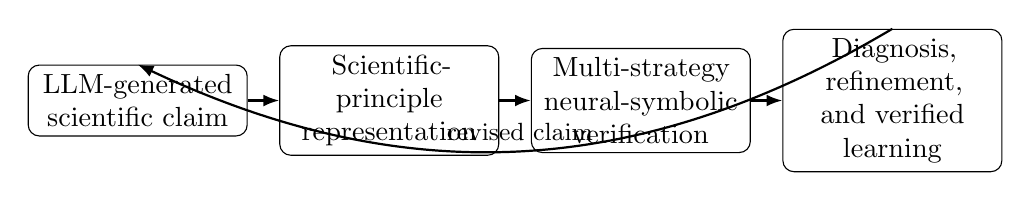
\begin{tikzpicture}[
    node distance=4mm,
    box/.style={draw, rounded corners, align=center, minimum height=9mm, text width=0.21\textwidth},
    arrow/.style={-{Latex[length=2mm]}, thick}
]
\node[box] (claim) {LLM-generated\\scientific claim};
\node[box, right=of claim] (repr) {Scientific-principle\\representation};
\node[box, right=of repr] (verify) {Multi-strategy\\neural-symbolic verification};
\node[box, right=of verify] (refine) {Diagnosis, refinement,\\and verified learning};
\draw[arrow] (claim) -- (repr);
\draw[arrow] (repr) -- (verify);
\draw[arrow] (verify) -- (refine);
\draw[arrow, bend left=28] (refine.north) to node[above, font=\small]{revised claim} (claim.north);
\end{tikzpicture}
\caption{Proposed framework. Scientific information is converted into explicit representations that support specialized verification mechanisms. Verification produces typed feedback that is used to diagnose and revise the claim.}
\label{fig:framework}
\end{figure}

\subsection*{Task 1: Representing Scientific Principles for Verification}

The first challenge is that scientific knowledge appears in heterogeneous forms. Some claims depend on evidence-backed facts (e.g., a material has a measured property); others depend on quantitative relations, relational rules, or logical constraints. A single unstructured text passage is therefore not an adequate representation for all verification operations.

We will develop a claim-driven scientific principle representation with four complementary forms: (1) \textbf{evidence-backed facts} linked to their source and provenance; (2) \textbf{quantitative relations} represented by variables, units, applicability conditions, and executable expressions; (3) \textbf{relational knowledge} represented as typed entities and relations; and (4) \textbf{logical constraints} that specify allowable or contradictory combinations of conditions. Rather than attempting to construct a complete scientific knowledge base, the system will begin with the target claim, decompose it into atomic verification units, retrieve the most relevant scientific sources, and extract only the principles required to test those units. This claim-driven design keeps the representation focused while allowing new domains to be incorporated as needed.

A neural semantic parser will map retrieved natural-language principles into the appropriate structured form. Because an executable representation can be syntactically valid but semantically wrong, we will explicitly test \emph{representation fidelity}: whether the structured form preserves the conditions and meaning of the source principle. We will combine source-to-representation consistency checks with type, unit, and constraint checks whenever they are available. The resulting representation will retain links to the original evidence so that every downstream verification result can be traced back to both the scientific principle and the source from which it was acquired.

\textbf{Research questions.} How much structure is needed to make heterogeneous scientific knowledge executable without creating a brittle knowledge-acquisition bottleneck? Can a common typed interface support facts, equations, relations, and constraints while preserving the semantics and applicability conditions of each?

\subsection*{Task 2: Multi-Strategy Neural-Symbolic Claim Verification}

The second challenge is that different scientific claims require different reasoning mechanisms. Asking one LLM to internally perform all reasoning makes it difficult to determine whether an error came from a missing fact, incorrect arithmetic, a violated constraint, or the use of the wrong scientific rule. We will instead develop a multi-strategy verifier in which a neural planner decomposes a target claim into verification steps and routes each step to a specialized reasoning mechanism.

For a quantitative principle, the system can translate the relevant relation into an executable expression and use a numerical or symbolic mathematics engine. For a logical rule or domain constraint, it can construct a first-order, logic-programming, or SMT representation and execute a solver, extending our prior work on explicit logical parsing and reasoning \citep{han2023clore}. For relational scientific facts, the system can reason over a structured knowledge graph; for evidence-backed factual claims, it can align the atomic claim with the retrieved source evidence. A claim that combines several kinds of reasoning will result in a composed verification plan rather than a single holistic judgment.

A key research problem is to distinguish \textbf{execution validity} from \textbf{semantic groundedness}. A program may run correctly while applying the wrong equation; a logic solver may return a valid conclusion from premises that do not apply to the scientific context. Recent work has highlighted this executable-but-ungrounded failure mode in structured STEM reasoning \citep{zi2026nsprm}. We will generalize this problem beyond fixed quantitative traces by explicitly representing applicability conditions and requiring the verifier to establish a link between the claim context, the selected principle, and the variables or entities used in execution. The output of each step will be a machine-checkable \emph{verification receipt}: the principle used, its source, the structured representation, the executor, the result, and the conditions under which the result is valid.

The system will also support self-debugging of intermediate representations. When a parser produces malformed code or logic, executor feedback will be used to repair the representation and retry the step. However, a successful execution will not itself be treated as proof of scientific correctness; semantic applicability remains an explicit check. This separation is important for avoiding false confidence from a deterministic but incorrectly formulated computation.

\textbf{Research questions.} How should a neural planner compose heterogeneous reasoning mechanisms while keeping the verification trace interpretable? When should a result be trusted as an executable check versus treated as a semantic judgment? Which combinations of neural and symbolic components generalize best to novel compositions of known scientific principles?

\subsection*{Task 3: Verification-Guided Diagnosis, Refinement, and Generalization}

A binary correct/incorrect label provides little information for correcting a complex scientific claim. Our third task will therefore convert verification receipts into typed diagnoses. We will distinguish at least four error classes: unsupported or contradictory facts, incorrectly selected or applied scientific rules, violated quantitative/logical constraints, and erroneous intermediate representations. The LLM will revise only the affected part of the claim using this feedback. A revised claim will be accepted only if the failed checks are resolved without invalidating components that previously passed, providing a simple form of backtracking against regressions. This extends the fine-grained philosophy of our prior FaithScore work, which decomposes generated outputs into atomic facts for separate verification \citep{jing2024faithscore}, from multimodal factuality to scientific reasoning.

We will further study whether verified representations can improve generalization before an error occurs. Scientific rules often permit controlled generation of new situations by changing variables, conditions, or combinations of principles. We will use the symbolic representations from Task 1 to construct counterfactual and compositional cases, execute them to obtain verified outcomes, and use these traces as training or preference signals. This component adapts the simulation-based synthetic-data idea from the original FAIGen proposal while making verification, rather than generic fine-tuning, the central source of supervision.

\section*{Evaluation and Measures of Success}

We will evaluate the framework across scientific domains containing complementary reasoning types, including quantitative physical/engineering relations, relational scientific knowledge, and logic- or constraint-based claims. Evaluation will combine existing scientific claim-verification resources with controlled challenge sets generated from known scientific principles. The controlled sets are important because they allow systematic variation of quantities, applicability conditions, and rule compositions while preserving a known ground truth.

The main metrics will be: (1) accuracy and recall of retrieving the principles required to verify a claim; (2) semantic fidelity and executability of the structured representations; (3) end-to-end claim-verification precision, recall, and F1; (4) accuracy of localizing the source and type of an error; (5) successful correction rate and no-regression rate after refinement; and (6) generalization to unseen values, conditions, and compositions of known principles. Baselines will include retrieval plus an end-to-end LLM judge, self-refinement without external verification, tool-augmented neural reasoning without explicit applicability checks, and symbolic-only variants. A primary success criterion is a substantial reduction in verification errors on compositional and previously unseen settings relative to the strongest end-to-end neural baseline, while preserving or improving performance on ordinary factual claims. We will also measure the added value of each representation and reasoning component through ablation studies.

\section*{Potential Impact on DAF and DoW Capabilities}

The Air Force and Space Force must make sense of heterogeneous information collected through different sources and at different levels of abstraction. Generative AI can help synthesize such information, but its use in scientific analysis, autonomy, and decision support depends on the ability to distinguish a fluent conclusion from one that is actually supported by domain knowledge. The proposed research directly connects bottom-up information extraction with top-down concept-driven reasoning: evidence and observations are converted into explicit representations, then evaluated using the scientific rules and constraints that govern the domain.

If successful, the project will provide fundamental methods for AI systems to combine multiple reasoning components, expose the basis of a generated scientific conclusion, identify the source of reasoning failures, and revise unsupported conclusions. These capabilities can improve information awareness, reduce the cognitive burden of manually checking complex AI-generated analyses, and make human-machine interaction more auditable. The project is not tied to a single mission application; instead, it develops general computational principles for reliable reasoning over heterogeneous knowledge that can support future DAF systems operating under unfamiliar or rapidly changing conditions.

\section*{Team and Development Plan}

PI Xinya Du will lead all research activities at UT Dallas. The project will involve graduate and undergraduate research students at UTD; no external collaborators or subawards are planned. The PI's prior work spans information extraction and knowledge representation, explicit logical reasoning over natural-language explanations \citep{han2023clore}, fine-grained hallucination evaluation \citep{jing2024faithscore}, and LLM-based scientific discovery. This combination provides the technical basis for connecting unstructured scientific information with explicit verification and iterative refinement.

The project will progress over three years. \textbf{Year 1} will develop the claim-driven scientific principle representation, build the first benchmark suite, and implement initial quantitative, factual, and relational verification modules. \textbf{Year 2} will focus on multi-strategy planning and composition, applicability checking, and self-debugging of symbolic representations; the main milestone will be an integrated verifier that produces step-level verification receipts across multiple reasoning types. \textbf{Year 3} will develop diagnosis and refinement, generate verified counterfactual/compositional training cases, and evaluate generalization under previously unseen conditions. The final deliverables will include research publications, evaluation datasets, and open-source implementations of the representation, verification, and refinement components.

\clearpage
\bibliographystyle{plainnat}
\IfFileExists{doug/references.bib}
  {\bibliography{doug/references}}
  {\bibliography{references}}

\end{document}
